\chapter{Week 3}
\section{Moving Average Processes}
Suppose $ X_t $ is stationary. Identify serial
dependence using ACF $ \hat{\rho}(h) $.
If the lines go out of the dotted blue boundaries,
namely $ \pm \displaystyle \frac{1.96}{\sqrt{T}} $,
within the ACF plot of $ \hat{\rho}(h) $, then we suspect serial dependence.

Posit
\[ X_t=g(W_t,W_{t-1},\ldots)=\sum_{\ell=0}^{\infty} \psi_\ell W_{t-\ell}\quad
    \text{[Linear Process]} \]
Not feasible to estimate infinitely many parameters
$ \set{\psi}_{\ell=0}^{\infty} $. Assume coefficients
arise from a \emph{parsimonious} linear model for $ X_t $.
\begin{Definition}{Moving average process}{}
    Suppose $ \set{W_t}_{\in\mathbf{Z}} $ is a strong
    white noise with $ \Var{W_t}=\sigma_W^2<\infty $.
    We say $ X_t $ is a \textbf{moving average process}
    of order $ q $ or $ \MA{q} $, if there exists
    $ \theta_1,\ldots,\theta_q\in\mathbf{R} $ with $ \theta_q\ne 0 $
    such that
    \[ X_t=W_t+\theta_1W_{t-1}+\cdots+\theta_q W_{t-q}=\sum_{\ell=0}^{q}
        \theta_\ell W_{t-\ell} \]
    where $ \theta_0=1 $. In other words, we've truncated
    the linear process representation at the level $ q $.
\end{Definition}
\begin{Definition}{Backshift operator}{}
    The \textbf{backshift operator}, $ B $, is defined
    by
    \[ B^j X_t=X_{t-j} \]
    $ B $ is assumed further to be linear in the sense
    that for $ a,b\in\mathbf{R} $
    \[ (a B^j+b B^k)X_t=
        a B^j X_t+b B^k X_t=a X_{t-j}+b X_{t-k} \]
\end{Definition}
\begin{Example}{}{}
    \begin{itemize}
        \item First difference of $ X_t $:
              \[ \nabla X_t=(1-B)X_t=X_t-B X_t=X_t-X_{t-1} \]
        \item Second difference of $ X_t $:
              \[ \nabla^2 X_t=(1-B)^2 X_t=(1-2B+B^2)X_t=X_t-2X_{t-1}+X_{t-2} \]
    \end{itemize}
\end{Example}
\begin{Definition}{Moving average operator}{}
    The \textbf{moving average operator} is defined by
    \[ \theta(B)=1+\theta_1 B+\theta_2 B^2+\cdots+\theta_q B^q \]
\end{Definition}
\begin{Definition}{Moving average polynomial}{}
    The \textbf{moving average polynomial} is defined as
    \[ \theta(x)=1+\theta_1 x+\cdots+\theta_q x^q \]
\end{Definition}
If $ X_t\sim\MA{q} $, then
\[ X_t=W_t+\theta_1W_{t-1}+\cdots+\theta_q W_{t-q}=\theta(B)W_t \]
which is a succinct expression defining $ \MA{q} $.
\subsection*{Properties of $ \MA{q} $ Processes}
\begin{enumerate}[(1)]
    \item $ \MA{0} $ process is a strong white noise.
    \item If $ X_t\sim\MA{q} $, then
          \[ \E{X_t}=\E[\bigg]{\sum_{\ell=0}^{q} \theta_\ell W_{t-\ell}}=0\quad (\theta_0=1) \]
          \[ \Var{X_t}=\E[\bigg]{\biggl(\sum_{\ell=0}^{q} \theta_\ell W_{t-\ell}\biggr)^{\!2}}=
              \sum_{\ell=0}^{q} \theta_\ell^2\sigma_W^2 \]
          \begin{align*}
              \gamma(h)
                                                               & =\Cov{X_t,X_{t+h}}                                                                                \\
                                                               & =\E[\bigg]{\biggl(\sum_{\ell=0}^{q} \theta_\ell W_{t-\ell}\biggr)
              \biggl(\sum_{k=0}^{q} \theta_k W_{t+h-k}\biggr)} &                                                                   & t-\ell=t+h-k\implies k=\ell+h \\
                                                               & =\begin{dcases}
                  \sigma_W^2\sum_{j=0}^{q-h} \theta_j \theta_{j+h} & 1\le h\le q \\
                  0                                                & h>q
              \end{dcases}
          \end{align*}
          Recall that $ \gamma(h)=\gamma(-h) $, so we will only display the values
          for $ h\ge 0 $. Note that $ \gamma(q) $ cannot be zero
          because $ \theta\ne 0 $. The cutting off of $ \gamma(h) $
          after $ q $ lags is the signature of the $ \MA{q} $ model.
          Therefore,
          \[ \rho(h)=\frac{\gamma(h)}{\gamma(0)} =
              \begin{dcases}
                  \frac{\sum_{j=0}^{q-h} \theta_j \theta_{j+h}}{\sum_{j=0}^{q} \theta_j^2} & 1\le h\le q \\
                  0                                                                        & h>q
              \end{dcases} \]
          \begin{Remark}{}{}
              By choosing $ \theta_1,\ldots,\theta_q $ appropriately, we can
              get any ACF we want $ \rho(h) $ where $ 1\le h\le q $.
          \end{Remark}
    \item If $ X_t\sim\MA{q} $, then $ X_t $ is $ q $-dependent.
\end{enumerate}
{\color{blue}In~\Cref{fig:maprocesses1}, let's look an example now of what a moving average process would
actually look like if we were to realize a moving average process.
On the top of~\Cref{fig:maprocesses1}, I've plotted a moving average process of order $ 0 $,
which is just a strong white noise. Then, as we progress down to
panel 2 and panel 3 I've calculated moving averages of orders $ 1 $ and
$ 2 $ based on this strong white noise sequence. In the second
panel, $ X_t=W_t+W_{t-1} $, so this is a moving average process
of order $ 1 $, in which $ \theta_1=1 $. In the third panel,
we have a moving average process of order $ 2 $,
in which $ X_t=W_t+W_{t-1}+W_{t-2} $, which is a
moving average process of order $ 2 $ where
$ \theta_1=\theta_2=1 $. One thing to observe when going
from a moving average process of order $ 0 $ to $ 2 $
is that the time series is getting ``smoother.''}

\begin{figure}[!htbp]
    \centering
    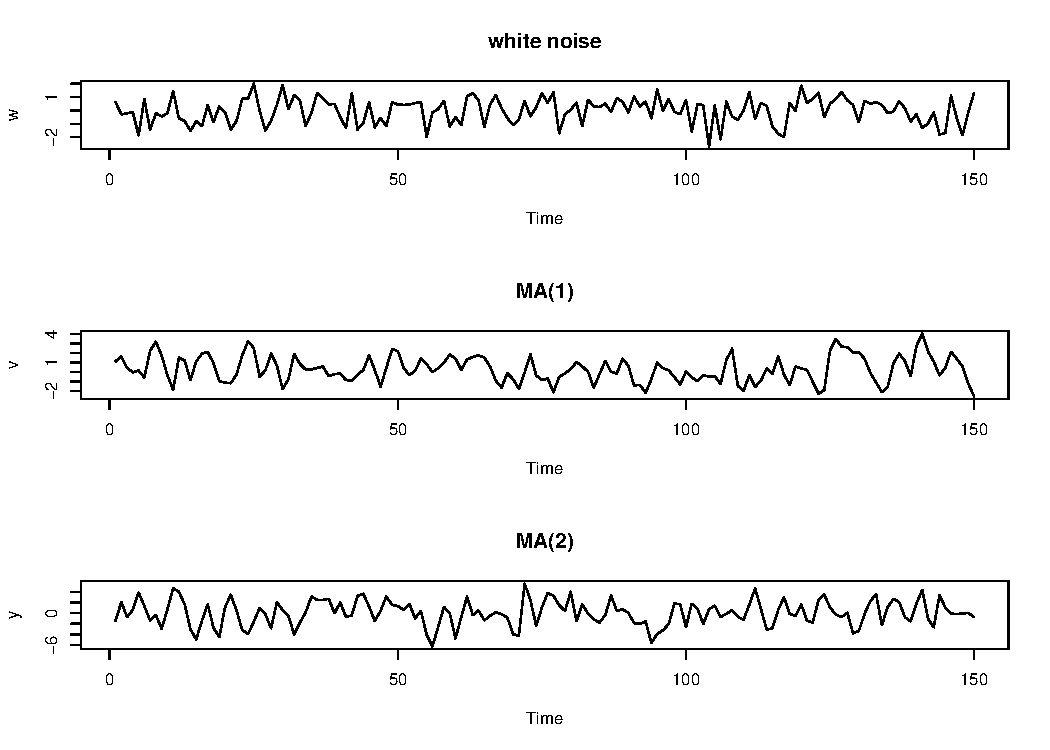
\includegraphics[width=\textwidth]{maprocesses1.pdf}
    \caption{Realizations of MA processes with coefficients equal to 1}\label{fig:maprocesses1}
\end{figure}
\begin{minted}{R}
# Figure 3.1
par(mfrow = c(3, 1))

ma0.sim <- arima.sim(list(order = c(0, 0, 0), ma = c()), n = 134)
plot(ma0.sim, ylab = "x", main = "white noise")

ma1.sim <- arima.sim(list(order = c(0, 0, 1), ma = c(1)), n = 134)
plot(ma1.sim, ylab = "v", main = (expression(MA(1) ~  ~  ~ theta[1] == 1)))

ma2.sim <-
  arima.sim(list(order = c(0, 0, 2), ma = c(1, 1)), n = 134)
plot(ma2.sim, ylab = "y", main = (expression(paste(
  MA(2), ~  ~  ~ theta[1], " = ",  theta[2], " = ", 1
))))
\end{minted}
In~\Cref{fig:maprocesses2}, the difference is apparent since
going from $ \MA{0} $ to $ \MA{1} $ shows that
$ \MA{1} $ has significant serial correlation
at lag $ 1 $. Similarly, for $ \MA{2} $
there is significant serial correlation
at lag $ 2 $.
\begin{figure}[!htbp]
    \centering
    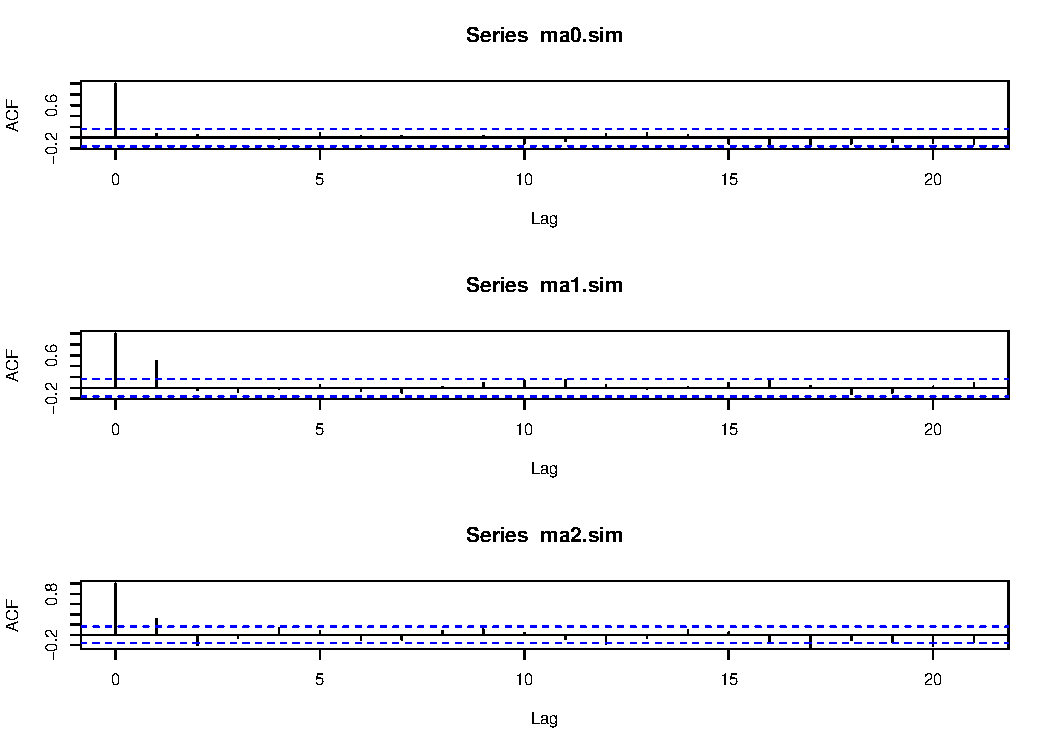
\includegraphics[width=\textwidth]{maprocesses2.pdf}
    \caption{ACF plots of corresponding moving average series.}\label{fig:maprocesses2}
\end{figure}
\begin{minted}{R}
# Figure 3.2
acf(ma0.sim)
acf(ma1.sim)
acf(ma2.sim)    
\end{minted}
\section{Autoregressive Processes}
\begin{Definition}{Autoregressive process}{}
    Suppose $ \set{W_t}_{t\in\mathbf{Z}} $ is a strong
    white noise with $ \Var{W_t}=\sigma_W^2<\infty $. We say
    $ X_t $ is an \textbf{autoregressive process}
    of order $ 1 $, or $ \AR{1} $, if there
    exists a constant $ \phi $ such that
    \[ X_t=\phi X_{t-1}+W_t\quad (t\in\mathbf{Z}) \]
    Using the backshift operator, this may also be expressed as
    \[ (1-\phi B)X_t=W_t \]
\end{Definition}
\subsection*{Interpretation}
\textbf{Prediction}: Form a linear model (regression)
predicting $ X_t $ as
\[ X_t=\phi X_{t-1}+W_t \]
where $ X_t $ is the dependent variable
and $ X_{t-1} $ is the covariant/independent variable.

\textbf{Markov Property}:
\[ X_t\mid (X_{t-1},X_{t-2},\ldots)=X_t\mid X_{t-1} \]
\textbf{Question}: Does there exist a stationary process
$ X_t $ satisfying the following?
\[ X_t=\phi X_{t-1}+W_t \]
Let's see.
\begin{align*}
    X_t
     & =\phi X_{t-1}+W_t                                                                                           \\
     & =\phi(\phi X_{t-2}+W_{t-1})+W_t                                                                             \\
     & =\phi^2X_{t-2}+\phi W_{t-1}+W_t                                                                             \\
     & \vdotswithin{=}                                           &  & k\text{ times}                               \\
     & =\textstyle\phi^k X_{t-k}+\sum_{j=0}^{k-1} \phi^j W_{t-j} &  & \text{if $ \abs{\phi}>1 $, the sum diverges} \\
\end{align*}
Suppose $ \abs{\phi}<1 $, then
\[ \xrightarrow[k\to\infty]{L^2\text{-sense}}0+
    \sum_{j=0}^{\infty} \phi^j W_{t-j} \]
which is a causal linear process. Moreover, if
$ X_t=\sum_{j=0}^{\infty} \phi^j W_{t-j} $, then
$ X_t $ is strictly stationary, and
\begin{align*}
    X_t
     & =\sum_{j=0}^{\infty} \phi^j W_{t-j}                           \\
     & =\sum_{j=1}^{\infty}\phi^j W_{t-j}+W_t                        \\
     & =\phi \sum_{j=1}^{\infty} \phi^{j-1}W_{t-j}+W_t &  & j\to j-1 \\
     & =\phi \sum_{j=0}^{\infty} \phi^j W_{t-1-j}+W_t                \\
     & =\phi X_{t-1}+W_t
\end{align*}
Therefore, $ X_t $ satisfies $ \AR{1} $ equation.
\begin{Theorem}{}{}
    If $ \abs{\phi}<1 $, then there exists a strictly stationary
    and causal linear process $ X_t $ such that
    \[ X_t=\phi X_{t-1}+W_t \]
\end{Theorem}
What if $ \abs{\phi}>1 $? If $ X_t=\phi X_{t-1}+W_t $ for $ t\in\mathbf{Z} $,
then that implies
\begin{align*}
    X_t
     & =\phi^{-1}X_{t+1}-\phi^{-1}W_{t+1}                                                           \\
     & =\phi^{-1}\bigl(\phi^{-1}X_{t+1}-\phi^{-1}W_{t+1}\bigr)-\phi^{-1}W_{t+1}                     \\
     & \vdotswithin{=}                                                          &  & k\text{ times} \\
     & =\textstyle\phi^{-k}X_{t+k}-\sum_{j=1}^{k-1} \phi^{-j}W_{t+j}
\end{align*}
Therefore,
\[ X_t=\frac{X_{t+k}}{\phi^k} -\sum_{j=1}^{k-1} \frac{W_{t+j}}{\phi^j}
    \xrightarrow[k\to\infty]{L^2\text{-sense}}-\sum_{j=1}^{\infty} \frac{W_{t+j}}{\phi^j}   \]
since $ \displaystyle \sum_{j=1}^{\infty} \frac{1}{\phi^j} <\infty $.
This sequence is strictly stationary since it is a Bernoulli shift.
However, what we have derived is not desirable as this model is
future dependent, normally we try to avoid this.

What if $ \abs{\phi}=1 $? In this case we claim that
there is no stationary process such that $ X_t=\phi X_{t-1}+W_t $. Let's prove this.
Suppose $ \abs{\phi}=1 $. If $ X_t=X_{t-1}+W_{t} $, then
\[ X_t=\sum_{j=1}^{t} W_j+X_0\quad\text{(by iterating)}
    \implies X_t-X_0=\sum_{j=1}^{t} W_j\quad\text{[Random Walk]} \]
Now, $ \abs[\big]{\Cov{X_t,X_0}}^2\le \Var{X_t}\Var{X_0}=\bigl(\Var{X_0}\bigr)^2 $,
so we get
\[ \abs[\big]{\Cov{X_t,X_0}}\le \sqrt{\Var{X_t}\Var{X_0}}=\sqrt{\bigl(\Var{X_0}\bigr)^2}=\Var{X_0} \]
Therefore, $ -2\Cov{X_t,X_0}\le 2\abs[\big]{\Cov{X_t,X_0}}\le 2\Var{X_0} $. Finally,
\[ \Var{X_t-X_0}=\Var{X_t}+\Var{X_0}-2\Cov{X_t,X_0}\le 4\Var{X_0} \]
where in the last inequality we used the fact that $ X_t $ is stationary.
Furthermore,
\[ \Var[\bigg]{\sum_{j=1}^{t} W_j}=t\sigma_W^2\xrightarrow{t\to\infty}\infty \]
\subsection*{Properties of Causal $ \AR{1} $ for $ \abs{\phi}<1 $}
\begin{enumerate}[(1)]
    \item The span of dependence of $ X_t $ is ``infinite''
          \[ X_t=\sum_{\ell=0}^{\infty} \phi^\ell W_{t-\ell} \]
    \item ACF.\@
          \[ \Var{X_t}=\E[\bigg]{\biggl(\sum_{\ell=0}^{\infty}\phi^\ell W_{t-\ell} \biggr)^{\!2}}
              =\sum_{\ell=0}^{\infty} \phi^{2\ell}\sigma_W^2=\frac{\sigma_W^2}{1-\phi^2}  \]
          \begin{align*}
              \gamma(h)
               & =\Cov{X_t,X_{t+h}}                                                                                                      \\
               & =\E[\bigg]{\biggl(\sum_{\ell=0}^{\infty} \phi^\ell W_{t-\ell}\biggr)\biggl(\sum_{k=0}^{\infty} \phi^k W_{t+h-k}\biggr)} \\
               & =\sum_{\ell=0}^{\infty} \phi^\ell \phi^{\ell+h}\sigma_W^2                                                               \\
               & =\phi^h \sum_{\ell=0}^{\infty} \phi^{2\ell}\sigma_W^2                                                                   \\
               & =\phi^h \biggl(\frac{\sigma_W^2}{1-\phi^2} \biggr)
          \end{align*}
          where in the first sum we let $ t-\ell=t+h-k $ and in the second sum
          we let $ k=\ell+h $ for $ \ell=0,1,2,\ldots $. Hence,
          \[ \rho(h)=\frac{\gamma(h)}{\gamma(0)} =\phi^h\quad(h\ge 0) \]
          Note: this decays geometrically in the lag parameter.
\end{enumerate}
\begin{minted}{R}
# Figure 3.3
ar0.sim <- arima.sim(list(order = c(1, 0, 0), ar = c(0.5)), n = 134)
plot(ar0.sim, ylab = "x", main = (expression(AR(1) ~  ~  ~ phi[1] == 0.5)))

ar1.sim <- arima.sim(list(order = c(1, 0, 0), ar = c(0.9)), n = 134)
plot(ar1.sim, ylab = "y", main = (expression(AR(1) ~  ~  ~ phi[1] == 0.9)))

ar2.sim <-
  arima.sim(list(order = c(1, 0, 0), ar = c(-0.9)), n = 134)
plot(ar2.sim, ylab = "z", main = (expression(AR(1) ~  ~  ~ phi[1] == -0.9)))

# Figure 3.4
acf(ar0.sim)
acf(ar1.sim)
acf(ar2.sim)    
\end{minted}
\begin{figure}[!htbp]
    \centering
    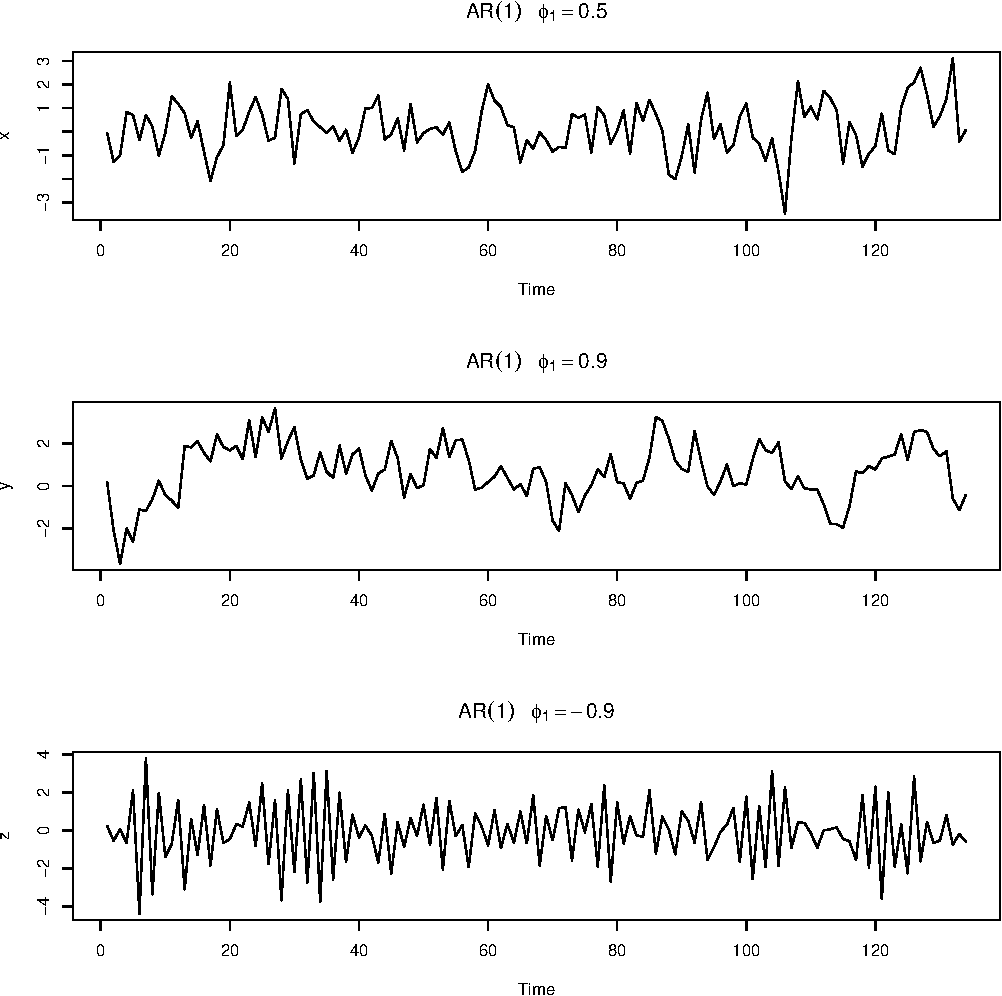
\includegraphics[width=\textwidth]{arprocesses1.pdf}
    \caption{Realizations of $ \AR{1} $ processes}\label{fig:arprocesses1}
\end{figure}
\begin{figure}[!htbp]
    \centering
    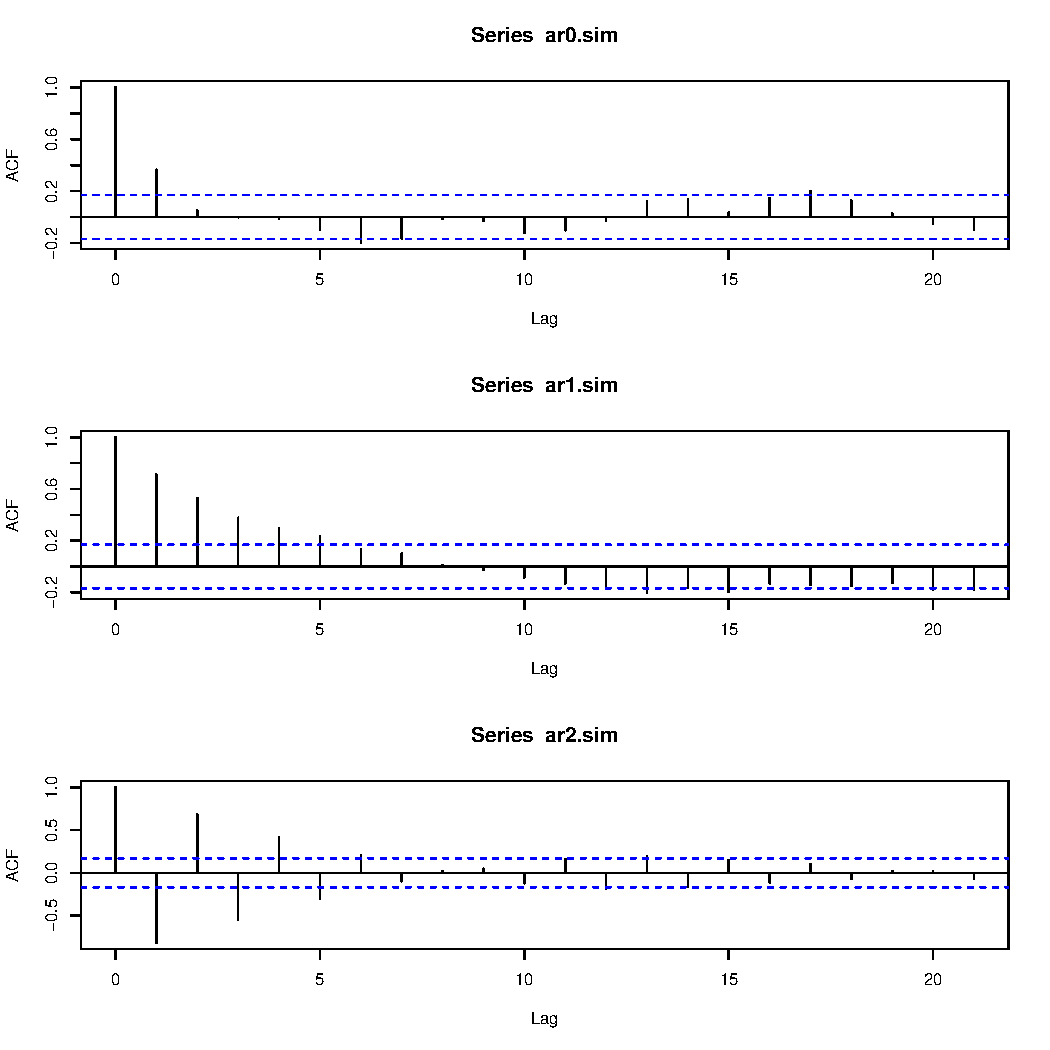
\includegraphics[width=\textwidth]{arprocesses2.pdf}
    \caption{Corresponding ACF plots}\label{fig:arprocesses2}
\end{figure}
\begin{Definition}{Autoregressive process, Autoregressive polynomial}{}
    We say $ X_t $ follows an \textbf{autoregressive process} of order $ p $,
    or $ \AR{p} $,
    if there exists coefficients $ \phi_1,\ldots,\phi_p\in\mathbf{R} $
    with $ \phi_p\ne 0 $ such that
    \[ X_t=\phi_1X_{t-1}+\cdots+\phi_p X_{t-p}+W_t \]
    We also define the \textbf{autoregressive polynomial} to be
    \[ \phi(x)=1-\phi_1 x-\cdots-\phi_p x^p \]
    $ X_t\sim \AR{p} $ if $ \phi(B)X_t=W_t $.
\end{Definition}
\section{ARMA Processes}
We've seen the moving average polynomial:
\[ \theta(x)=1+\theta_1 x+\cdots+\theta_q x^q\quad(\theta_q\ne 0) \]
and the autoregressive polynomial:
\[ \phi(x)=1-\phi_1 x-\cdots - \phi_p x^p\quad(\phi_p\ne 0) \]
If $ W_t\sim $ strong white noise
\[ X_t=\theta(B)W_t\quad(X_t\sim \MA{q}) \]
\[ \phi(B)X_t=W_t\quad(X_t\sim\AR{p}) \]
Why not combine the two?
\begin{Definition}{Autoregressive moving average}{}
    Given a strong white noise sequence $ W_t $, we say
    that $ X_t $ is an \textbf{autoregressive moving average} process
    of orders $ p $ and $ q $, or $ \ARMA{p,q} $, if $ X_t $ is stationary
    and
    \[ \phi(B)X_t=\theta(B)W_t \]
    \[ \phi(z)=1-\phi_1 z-\cdots - \phi_p z^p\quad (\phi_p\ne 0) \]
    \[ \theta(z)=1+\theta_1 z+\cdots+\theta_q z^q \quad (\theta_q\ne 0) \]
    This implies that the model is
    \[ X_t=\phi_1X_{t-1}+\cdots+\phi_p X_{t-p}+
        W_t+\theta_1 W_{t-1}+\cdots+\theta_q W_{t-q} \]
\end{Definition}
Using ARMA models to model autocorrelation: ARMA combines the
following two points.
\begin{itemize}
    \item $ \MA{q} $: ACF may be specified at lags $ 1,\ldots,q $
    \item $ \AR{p} $: ACF has geometric decay/oscillations
\end{itemize}
\begin{Remark}{Parameter redundancy}{}
    Consider $ X_t=W_t $ where $ X_t\sim \MA{0} $, then
    \[ 0.5 X_{t-1}=0.5 W_{t-1} \]
    Therefore,
    \[ X_t-0.5 X_{t-1}=W_{t}-0.5W_{t-1}\implies X_t\sim \ARMA{1,1} \]
    \[ \phi(z)=1-0.5z\implies \text{zero of $\phi$ is }z_0=2 \]
    \[ \theta(z)=1-0.5z\implies \text{zero of $\theta$ is }z_0=2 \]
    Parameter redundancy manifests as shared zeros in $ \phi $
    and $ \theta $. We always assume the models are ``reduced''
    by factoring and diving away common zeros in $ \phi $.
\end{Remark}
\begin{Definition}{Causal ARMA}{}
    We say an $ \ARMA{p,q} $ is \textbf{causal} if there exists $ \set{X_t}_{t\in\mathbf{Z}} $
    satisfying $ \phi(B)X_t=\theta(B)W_{t}$ and
    \[ X_t=\sum_{\ell=0}^{\infty} \psi_\ell W_{t-\ell}=\psi(B)W_t \quad\text{[Causal Linear Process Solution]} \]
    where $ \psi(B)=\sum_{\ell=0}^{\infty} \psi_\ell B^\ell $
    and $ \sum_{\ell=0}^{\infty} \abs{\psi_\ell}<\infty $ with
    $ \psi_0=1 $.
\end{Definition}
\begin{Definition}{Invertible ARMA}{}
    An $ \ARMA{p,q} $ is \textbf{invertible} if there exists $ \set{X_t}_{t\in\mathbf{Z}} $ satisfying
    $ \phi(B)X_t=\theta(B)W_t $ and
    \[ W_t=\sum_{\ell=0}^{\infty} \pi_\ell X_{t-\ell}=\pi(B)X_t \]
    where $ \pi(B)=\sum_{\ell=0}^{\infty} \pi_\ell B^\ell $
    and $ \sum_{\ell=0}^{\infty} \abs{\pi_\ell}<\infty $ with
    $ \pi_0=1 $.
\end{Definition}
\begin{Remark}{}{}
    Causality $ + $ Invertibility $ \implies  $ Information
    in $ \set{X_t}_{t\le T} $ is the same as Information in
    $ \set{W_t}_{t\le T} $ where $ \set{X_t}_{t\le T} $ is
    an observed time series.
\end{Remark}
\begin{Theorem}{Causality}{}
    By the fundamental theorem of algebra, the autoregressive
    polynomial $ \phi(z) $ has $ p $ roots,
    say $ z_1,\ldots,z_p\in\mathbf{C} $. If
    $ \displaystyle  \rho=\min_{1\le j\le p}\abs{z_j}>1 $,
    then there exists a stationary and causal $ X_t $
    to the ARMA equations: $ \phi(B)X_t=\theta(B)W_t $.
    \[ X_t=\sum_{\ell=0}^{\infty} \psi_\ell W_{t-\ell} \]
    The coefficients $ \set{\psi_\ell}_{\ell=0}^\infty $
    satisfy
    \[ \sum_{\ell=0}^{\infty} \abs{\psi_\ell}<\infty \]
    in fact,
    \[ \abs{\psi_\ell}\le \frac{1}{\rho^\ell}  \]
    which is the geometric decay. Also,
    \[ \psi(z)=\sum_{\ell=0}^{\infty}\psi_\ell z^\ell=\frac{\theta(z)}{\phi(z)}
        \quad(\abs{z}\le 1)  \]
    In essence,
    \[ X_t=\frac{\theta(B)}{\phi(B)}W_t=\sum_{j=0}^{\infty} \psi_j B^j W_t  \]
    Key: $ \displaystyle \frac{1}{\phi(z)}=\sum_{j=0}^{\infty}
        \phi_j z^j $ where $ \abs{z}\le 1 $ so $ \displaystyle \frac{1}{\phi} $ has a convergent power
    series representation for $ \abs{z}\le 1 $.
\end{Theorem}
\begin{Theorem}{Invertibility}{}
    If $ z_1,\ldots,z_q $ are the zeros
    of $ \theta(z) $ and $ \displaystyle \min_{1\le i\le q}\abs{z_i}>1 $,
    then $ X_t $ is invertible,
    \[ W_t=\sum_{\ell=0}^{\infty} \pi_\ell X_{t-\ell} \]
    Coefficients $ \set{\pi_\ell}_{\ell=0}^\infty $ satisfy
    \[ \pi(z)=\sum_{\ell=0}^{\infty} \pi_\ell z^\ell =\frac{\phi(z)}{\theta(z)}
        \quad (\abs{z}\le 1)  \]
\end{Theorem}
\underline{Moral}: When we look for coefficients
$ \phi_1,\ldots,\phi_p,\theta_1,\ldots,\theta_q $,
we want to do so in such a way that
\[ \phi(z),\theta(z)\ne 0\quad(\abs{z}\le 1) \]
\section{ARMA Process Examples and ACF}
\begin{Example}{}{}
    Consider the $ \ARMA{2,2} $ model
    \[ X_t= \frac{1}{4}X_{t-1} + \frac{1}{8} X_{t-2} + W_t - \frac{5}{6}W_{t-1} +\frac{1}{6}W_{t-2} \]
    Questions:
    \begin{itemize}
        \item Is there a stationary and causal solution to $X_t$?
        \item Is it invertible?
        \item Is there parameter redundancy?
    \end{itemize}
    AR polynomial:
    \[ \phi(z)=1-\frac{1}{4}z- \frac{1}{8}z^2  \]
    MA polynomial:
    \[ \theta(z)= 1-\frac{5}{6}z + \frac{1}{6}z^2\]
    Roots for $\phi$:
    \[ \frac{2 \pm \sqrt{4+ 4(8)}}{-2} =-1 \pm 3=-4,2 \]
    Roots for $\theta$: $ 2,3 $
    \[ \implies \phi(z)= -\frac{1}{8}(z+4)(z-2), \quad  \theta(z) = \frac{1}{6}(z-2)(z-3)\]
    Note that $\phi (z)$ and $\theta (z)$ share common $(z-2)$ which indicates
    that the parameters are redundant.
    Therefore, $X_t$ satisfies an $ \ARMA{1,1} $ with
    \[\phi(z)=-\frac{1}{8}(z+4), \quad \theta(z)= \frac{1}{6}(z-3)\]
    Since the roots of $\phi$ and $\theta$ are
    outside the unit circle in $\mathbb{C}$, $X_t$ is
    stationary, causal, and invertible.
\end{Example}
\begin{Example}{}{}
    Suppose
    \[ X_t =-\frac{1}{4} X_{t-1}+W_t-\frac{1}{3}W_{t-1}\]
    where $X_t \sim \ARMA{1,1}$.
    \[\phi(z)=1+\frac{1}{4}z \implies \text{Root is $-4$.}\]
    So $X_t$ is stationary and causal, and can be represented as a linear process:
    \[X_t= \sum^{\infty}_{\ell=0} \psi_\ell W_{t-\ell} \]
    We need to calculate the coefficients $\psi_\ell$.

    We know
    \[\psi(z)= \sum^{\infty}_{\ell=0} \psi_\ell z^\ell = \frac{\theta(z)}{\phi(z)}\quad (\abs{z}\leq 1)  \]
    \[\implies \psi(z)\phi(z)=\theta(z) \]
    Note that both $ \psi(z)\phi(z) $ and $ \theta(z) $ are power series, therefore
    we can calculate $ \psi_\ell $ by matching coefficients.
    \begin{itemize}
        \item $ \displaystyle \phi(z)=1+ \frac{1}{4}z $
        \item $ \displaystyle  \theta(z)= 1-\frac{1}{3}z $
        \item $ \psi(z)\phi(z)=\theta(z) $
    \end{itemize}
    Let's compute it.
    \begin{align*}
        z^0    :\quad & \psi_0=1                                                                                          \\
        z^1    :\quad & \frac{\psi_0}{4}+\psi_1=-\frac{1}{3}  &  & \implies \psi_1=-\frac{7}{12}                          \\
        z^2    :\quad & \frac{\psi_1}{4}+\psi_2 = 0           &  & \implies \psi_2=\frac{7}{12} \biggl(\frac{1}{4}\biggr) \\
        \vdots \quad  &                                                                                                   \\
        z^\ell :\quad & \frac{\psi_{\ell-1}}{4} + \psi_\ell=0 &  & \implies
        \psi_\ell= (-1)^{\ell}\frac{7}{12}\biggl(\frac{1}{4}\biggr)^{\ell-1}\quad(\ell\ge 1)
    \end{align*}
    Simplifying,
    \[ \psi_j=
        \begin{dcases}
            1                                        & j=1    \\
            \frac{7}{3} \biggl(-\frac{1}{4}\biggr)^j & j\ge 1
        \end{dcases} \]
    We can automate $ \psi_j $ in R with \texttt{ARMAtoMA()}.
    \begin{minted}{R}
    library(astsa)
    ARMAtoMA(ar=-1/4, ma=-1/3, 10)
    \end{minted}
    If $X_t$ is a stationary and causal solution to the $\ARMA{p,q}$ model.
    \[X_t = \sum^{\infty}_{j=0} \psi_j W_{t-j}\]
    \[\gamma_X(h) =
        \E{X_t X_{t+h}}= \E[\bigg]{\biggl(\sum^{\infty}_{j=0}\psi_j W_{t-j}\biggr)\biggl(\sum^{\infty}_{k=0} \psi_k W_{t+h-k}\biggr)} \]
    Note that
    \[t-j= t+h-k, \implies k=h+j,\, j=0,1,2,\ldots\quad  \E{X^2_{t-j}}=\sigma_W^2\]
    Therefore,
    \[\gamma_X(h) =\sigma_W^2 \sum^{\infty}_{j=0} \psi_j \psi_{j+h} \]
    We can automate $\gamma_X(h)$ in R with \texttt{ARMAacf()}.

    For $ h\ge 1 $, we have
    \begin{align*}
        \gamma_X(h)
         & =\sum_{j=0}^{\infty} \psi_j\psi_{j+h}                                                                               \\
         & =\psi_0\psi_h+\sum_{j=1}^{\infty}\psi_j\psi_{j+1}                                                                   \\
         & =\frac{7}{3} \biggl(-\frac{1}{4}\biggr)^{h}+
        \sum_{j=1}^{\infty} \Biggl[\frac{7}{3}\biggl(-\frac{1}{4}\biggr)^{j}\frac{7}{3}\Bigl(-\frac{1}{4} \biggr)^{j+1}\Biggr] \\
         & =\frac{91}{135}(-1)^h 4^{1-h}
    \end{align*}
    Then,
    \begin{align*}
        \gamma_X(0)
         & =\sum_{j=0}^{\infty} \psi_j^2                                     \\
         & =(1)^2+\sum_{j=1}^{\infty} \psi_j^2                               \\
         & =1+\sum_{j=1}^{\infty} \frac{7}{3} \biggl(-\frac{1}{4}\biggr)^{j} \\
         & =\frac{184}{135}
    \end{align*}
    Therefore, the ACF for $ h\ge 1 $ is given by
    \[ \rho_X(h)=\begin{dcases}
            1                                                                                                                   & h=0    \\
            \frac{\gamma_X(h)}{\gamma_X(0)}=\frac{\frac{91}{135}(-1)^h 4^{1-h}}{\frac{184}{135}}=\frac{91}{23} (-1)^h 2^{-2h-1} & h\ge 1
        \end{dcases}
    \]
    Let's verify this in R.
    \begin{minted}{R}
round(ARMAacf(ar = -1 / 4, ma = -1 / 3, 5), 6)
h <- seq(1, 10, by = 1)
round((91 / 23) * (-1) ^ h * 2 ^ (-2 * h - 1), 6)
\end{minted}
    \textbf{Output}:
    \begin{minted}{R}
        0         1         2         3         4         5
 1.000000 -0.494565  0.123641 -0.030910  0.007728 -0.001932

          -0.494565  0.123641 -0.030910  0.007728 -0.001932
\end{minted}
    As we can see, this is correct.
\end{Example}
